\documentclass[tikz,border=3mm,multi=tikzpicture]{standalone}
\usepackage[utf8]{inputenc}
\usepackage[T1]{fontenc}
\usepackage{helvet}
\renewcommand{\familydefault}{\sfdefault}
\usepackage{tikz}
\usetikzlibrary{angles,quotes,calc,intersections}
\begin{document}

\tikzset{every node/.append style={font=\sffamily\small}}
% TikZ 1
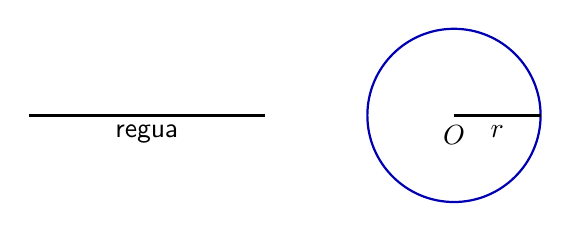
\begin{tikzpicture}[scale=1]
\coordinate (A) at (0,0); \coordinate (B) at (3,0);
\draw[thick] (A)--(B);
\node[below] at (1.5,0) {regua};
\coordinate (O) at (5.4,0);
\draw[blue!70!black,thick] (O) circle (1.1);
\draw[thick] (O)--(6.5,0);
\node[below] at (O) {$O$};
\node[below] at (5.95,0) {$r$};
\end{tikzpicture}
% TikZ 2
\begin{tikzpicture}[scale=1]
\coordinate (A) at (0,0); \coordinate (B) at (3,0); \coordinate (C) at (1.5,2.598);
\draw[thick] (A)--(B)--(C)--cycle;
\draw[blue!70!black,dashed] (A) circle (3);
\draw[blue!70!black,dashed] (B) circle (3);
\foreach \p/\pos in {A/below left,B/below right,C/above}{\node[\pos] at (\p) {$\p$};}
\end{tikzpicture}


% TikZ 3
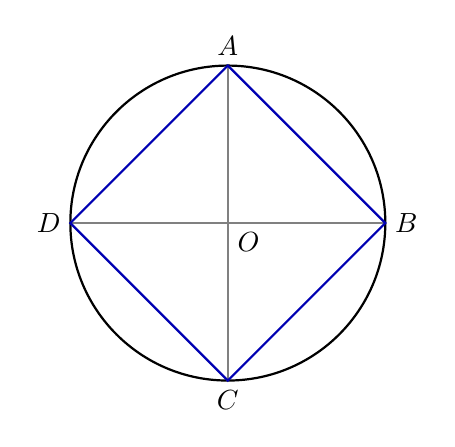
\begin{tikzpicture}[scale=1]
\coordinate (O) at (0,0); \coordinate (A) at (0,2); \coordinate (B) at (2,0); \coordinate (C) at (0,-2); \coordinate (D) at (-2,0);
\draw[thick] (O) circle (2);
\draw[gray,thick] (A)--(C);
\draw[gray,thick] (D)--(B);
\draw[thick,blue!70!black] (A)--(B)--(C)--(D)--cycle;
\foreach \p/\pos in {A/above,B/right,C/below,D/left,O/below right}{\node[\pos] at (\p) {$\p$};}
\end{tikzpicture}
% TikZ 4
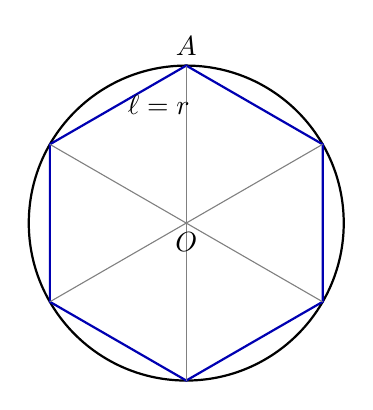
\begin{tikzpicture}[scale=1]
\coordinate (O) at (0,0);
\draw[thick] (O) circle (2);
\foreach \k in {1,...,6}{\coordinate (P\k) at ({90+60*(\k-1)}:2);}
\draw[thick,blue!70!black] (P1)--(P2)--(P3)--(P4)--(P5)--(P6)--cycle;
\foreach \k in {1,...,6}{\draw[gray] (O)--(P\k);}
\node[below] at (O) {$O$};
\node[above] at (P1) {$A$};
\node[right] at ($(P1)!0.5!(P2)$) {$\ell=r$};
\end{tikzpicture}
\end{document}
